\documentclass{article}
\usepackage{graphicx, tikz-cd, float, titlepic, booktabs} % Required for inserting images
\usepackage{pgfplots}
\usepackage{multicol}
\usepackage{makecell}
\pgfplotsset{compat=1.15}
\usepackage{mathrsfs}
\usetikzlibrary{arrows}
\usepackage{amsmath, amssymb, amsthm, amsfonts, siunitx, physics, gensymb}
\AtBeginDocument{\RenewCommandCopy\qty\SI}
\usepackage[version=4]{mhchem}
\usepackage[most,many,breakable]{tcolorbox}
\usepackage{xcolor, fancyhdr, varwidth}
\usepackage[Glenn]{fncychap}
%Options: Sonny, Lenny, Glenn, Conny, Rejne, Bjarne, Bjornstrup
\usepackage{hyperref, cleveref}
\usepackage{icomma, enumitem} %comma as decimal and continue enumerate with [resume]
\usepackage{plimsoll} %use standard state symbol with \stst
\usepackage[danish]{babel}
\renewcommand{\cellalign}{cl}
\renewcommand{\theadalign}{cl}
\renewcommand\theadfont{\bfseries}
%%%%%%%%%%%%%%%%%%%%%%%%%%%%%%
% SELF MADE COLORS
%%%%%%%%%%%%%%%%%%%%%%%%%%%%%%
\definecolor{myg}{RGB}{56, 140, 70}
\definecolor{myb}{RGB}{45, 111, 177}
\definecolor{myr}{RGB}{199, 68, 64}
\definecolor{mytheorembg}{HTML}{F2F2F9}
\definecolor{mytheoremfr}{HTML}{00007B}
\definecolor{mylenmabg}{HTML}{FFFAF8}
\definecolor{mylenmafr}{HTML}{983b0f}
\definecolor{mypropbg}{HTML}{f2fbfc}
\definecolor{mypropfr}{HTML}{191971}
\definecolor{myexamplebg}{HTML}{F2FBF8}
\definecolor{myexamplefr}{HTML}{88D6D1}
\definecolor{myexampleti}{HTML}{2A7F7F}
\definecolor{mydefinitbg}{HTML}{E5E5FF}
\definecolor{mydefinitfr}{HTML}{3F3FA3}
\definecolor{notesgreen}{RGB}{0,162,0}
\definecolor{myp}{RGB}{197, 92, 212}
\definecolor{mygr}{HTML}{2C3338}
\definecolor{myred}{RGB}{127,0,0}
\definecolor{myyellow}{RGB}{169,121,69}
\definecolor{myexercisebg}{HTML}{F2FBF8}
\definecolor{myexercisefg}{HTML}{88D6D1}
%%%%%%%%%%%%%%%%%%%%%%%%%%%%%%%%%%%%%%%%%%%%%%%%%%%%%%%%%%%%%%%%%%%%%%
% Box environments for theorems and problems
%%%%%%%%%%%%%%%%%%%%%%%%%%%%%%%%%%%%%%%%%%%%%%%%%%%%%%%%%%%%%%%%%%%%%
\setlength{\parindent}{1cm}
%================================
% Question BOX
%================================
\makeatletter
\newtcbtheorem{question}{Opgave}{enhanced,
	breakable,
	colback=white,
	colframe=myb!80!black,
	attach boxed title to top left={yshift*=-\tcboxedtitleheight},
	fonttitle=\bfseries,
	title={#2},
	boxed title size=title,
	boxed title style={%
			sharp corners,
			rounded corners=northwest,
			colback=tcbcolframe,
			boxrule=0pt,
		},
	underlay boxed title={%
			\path[fill=tcbcolframe] (title.south west)--(title.south east)
			to[out=0, in=180] ([xshift=5mm]title.east)--
			(title.center-|frame.east)
			[rounded corners=\kvtcb@arc] |-
			(frame.north) -| cycle;
		},
	#1
}{def}
\makeatother
%================================
% DEFINITION BOX
%================================

\newtcbtheorem[number within=section]{definition}{Definition}{enhanced,
	before skip=2mm,after skip=2mm, colback=red!5,colframe=red!80!black,boxrule=0.5mm,
	attach boxed title to top left={xshift=1cm,yshift*=1mm-\tcboxedtitleheight}, varwidth boxed title*=-3cm,
	boxed title style={frame code={
					\path[fill=tcbcolback]
					([yshift=-1mm,xshift=-1mm]frame.north west)
					arc[start angle=0,end angle=180,radius=1mm]
					([yshift=-1mm,xshift=1mm]frame.north east)
					arc[start angle=180,end angle=0,radius=1mm];
					\path[left color=tcbcolback!60!black,right color=tcbcolback!60!black,
						middle color=tcbcolback!80!black]
					([xshift=-2mm]frame.north west) -- ([xshift=2mm]frame.north east)
					[rounded corners=1mm]-- ([xshift=1mm,yshift=-1mm]frame.north east)
					-- (frame.south east) -- (frame.south west)
					-- ([xshift=-1mm,yshift=-1mm]frame.north west)
					[sharp corners]-- cycle;
				},interior engine=empty,
		},
	fonttitle=\bfseries,
	title={#2},#1}{def}

%================================
% NOTE BOX
%================================

\usetikzlibrary{arrows,calc,shadows.blur}
\tcbuselibrary{skins}
\newtcolorbox{note}[1][]{%
	enhanced jigsaw,
	colback=gray!20!white,%
	colframe=gray!80!black,
	size=small,
	boxrule=1pt,
	title=\textbf{Note:},
	halign title=flush center,
	coltitle=black,
	breakable,
	drop shadow=black!50!white,
	attach boxed title to top left={xshift=1cm,yshift=-\tcboxedtitleheight/2,yshifttext=-\tcboxedtitleheight/2},
	minipage boxed title=1.5cm,
	boxed title style={%
			colback=white,
			size=fbox,
			boxrule=1pt,
			boxsep=2pt,
			underlay={%
					\coordinate (dotA) at ($(interior.west) + (-0.5pt,0)$);
					\coordinate (dotB) at ($(interior.east) + (0.5pt,0)$);
					\begin{scope}
						\clip (interior.north west) rectangle ([xshift=3ex]interior.east);
						\filldraw [white, blur shadow={shadow opacity=60, shadow yshift=-.75ex}, rounded corners=2pt] (interior.north west) rectangle (interior.south east);
					\end{scope}
					\begin{scope}[gray!80!black]
						\fill (dotA) circle (2pt);
						\fill (dotB) circle (2pt);
					\end{scope}
				},
		},
	#1,
}
%================================
% EXAMPLE BOX
%================================
\newtcbtheorem[number within=section, use counter from=definition]{Example}{Example}
{%
	colback = myexamplebg
	,breakable
	,colframe = myexamplefr
	,coltitle = myexampleti
	,boxrule = 1pt
	,sharp corners
	,detach title
	,before upper=\tcbtitle\par\smallskip
	,fonttitle = \bfseries
	,description font = \mdseries
	,separator sign none
	,description delimiters parenthesis
}
{ex}
%================================
% THEOREM BOX
%================================

\tcbuselibrary{theorems,skins,hooks}
\newtcbtheorem[number within=section, use counter from=definition]{Theorem}{Theorem}
{%
	enhanced,
	breakable,
	colback = mytheorembg,
	frame hidden,
	boxrule = 0sp,
	borderline west = {2pt}{0pt}{mytheoremfr},
	sharp corners,
	detach title,
	before upper = \tcbtitle\par\smallskip,
	coltitle = mytheoremfr,
	fonttitle = \bfseries\sffamily,
	description font = \mdseries,
	separator sign none,
	segmentation style={solid, mytheoremfr},
}
{th}

%%%%%%%%%%%%%%%%%%%%%%%%%%%%%%%%%%%%%%%%%%%%%%%%%%%%%%%%%%%%%%%%%
% SELF MADE COMMANDS
%%%%%%%%%%%%%%%%%%%%%%%%%%%%%%
\newcommand{\sol}{\setlength{\parindent}{0cm}\textbf{\textit{Løsning:}}\setlength{\parindent}{1cm}}
%%%%%%%%%%%%%%%%%%%%%%%%%%%%%%%%%
\usepackage[tmargin=2cm,rmargin=1in,lmargin=1in,margin=0.85in,bmargin=2cm,footskip=.2in]{geometry}\pagestyle{fancy}
\lhead{Minrui Kevin Zhou 3.b}
\rhead{Aflevering 41}

\title{Aflevering 41\\
{\Large \textbf{3.b mat A}}}
\author{Kevin Zhou}
\date{\today}

\begin{document}
\maketitle
\newpage
\begin{question}{Normalfordelt stokastisk variabel}{}
 Tæthedsfunktionen for en normalfordelt stokastisk variabel $X$ er givet ved

$$f(x)=\frac{1}{\sqrt{2\pi}\cdot3}\cdot\mathrm{e}^{-\frac{1}{2}\cdot\left(\frac{x-10}{3}\right)^2}\:.$$
\end{question}
\sol \\
\textbf{a.}
For at finde middelværdien og spredningen for $X$, betragter vi den generelle tæthedsfunktionen for en stokastisk variabel med middelværdi $\mu $ og spredning $\sigma $:
\[
f(x)= \frac{1}{\sqrt{2 \pi } \cdot \sigma } \cdot e^{-\frac{1}{2} \cdot \left(\frac{x- \mu }{\sigma }\right)^2} 
\] 
Det er klart for $X$, at middelværdien må være $\mu =10$ og spredningen må være $\sigma = 3$. \\[1ex]
\textbf{b.}
Vi ser, at 
\begin{equation*}
\begin{split}
  P(7 \leq X \leq 13) &= P(10-3 \leq X \leq 10 + 3)\\
  &=P(\mu - \sigma \leq X \leq \mu + \sigma )
\end{split}
\end{equation*}
For en vilkårlig normalfordelt stokastisk variabel $X$ gælder der, at 
\[
P(\mu - \sigma \leq X \leq \mu + \sigma )\approx 68,27 \% 
\] 
Altså må sandsynligheden $P(7 \leq 10 \leq 13)$ være 68,27 \%. 

\begin{question}{Normalfordelt stokastisk variabel}{}
  En normalfordelt stokastisk variabel $X$ er givet ved $X \sim  N(6,0.7)$. 
  Tæthedsfunktionen for $X$ betegnes $f$. 
\end{question}
\sol \\
\textbf{a.}
Grafen for $f$ ses i \cref{fig:tæthed}. 
\begin{figure}[H]
\begin{center}
  \includegraphics[width=\textwidth]{tæthed.png}
\end{center}
\caption{Grafen for tæthedsfunktionen $f$ }
\label{fig:tæthed}
\end{figure}
\noindent\textbf{b.}
Vi beregner $\int_{5}^{8} f(x) \,dx $ med CAS (se \cref{fig:CASint}), og får 
\[
\int_{5}^{8} f(x) \,dx \approx 0,9213
\] 
Det fortæller om $X$, at $P(5 \leq X \leq 8)\approx 0,9213$.
\begin{figure}[H]
\begin{center}
  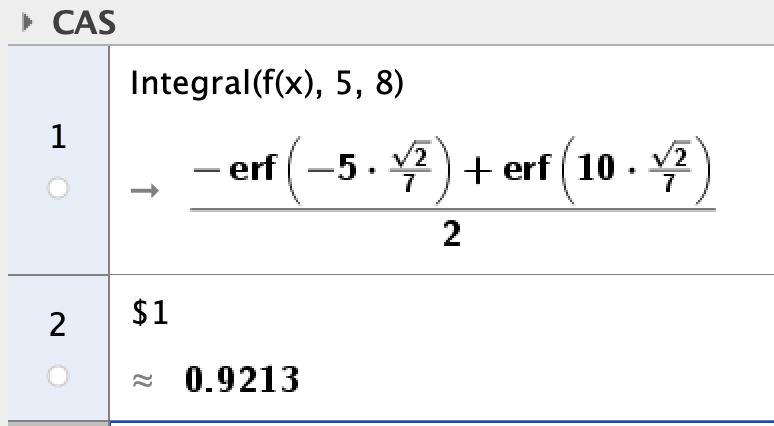
\includegraphics[width=0.5\textwidth]{CASint.png}
\end{center}
\caption{Integralet udregnet med CAS}
\label{fig:CASint}
\end{figure}
\begin{question}{Koncentration af hæmoglobin}{}
I en model kan koncentrationen af hæmoglobin i blodet hos kvinder beskrives ved en normalfordelt stokastisk variabel $X.$
Målt i mmol/L har $X$ middelværdien $\mu=8,4$ og spredningen $\sigma=0,55.$
\end{question}
\sol \\
\textbf{a.}
De normale udfald for $X$ er 
\begin{equation*}
\begin{split}
  [\mu - 2 \sigma; \mu + 2 \sigma ] &=[8,4 - 2 \cdot 0,55; 8,4 + 2 \cdot 0,55]\\
  &=[7,3;9,5]
\end{split}
\end{equation*}
Mængden af de normale udfald for $X$ er altså $[7,3;9,5]$.\\[1ex]
\textbf{b.}
For at bestemme sandsynligheden $P(X \leq 8,0)$, benytter vi CAS, hvilket ses i \cref{fig:CASleq8}.
\begin{equation*}
\begin{split}
  P(X \leq 8)&= \Phi \left(\frac{8- 8,4}{0,55}\right) \\
  &=\int_{-\infty }^{\frac{8-8,4}{0,55}} \frac{e^{- \frac{1}{2}} \cdot x ^2}{\sqrt{2 \pi } } \,dx \\
  &\approx 0,2335\\
  &=23,35 \%
\end{split}
\end{equation*}
Sandsynligheden for, at en tilfældigt udvalgt kvinde har en koncentration af hæmoglobin i blodet på højst $8,0 \;\unit{mmol/L} $ er altså 23,35 \%. 
\begin{figure}[H]
\begin{center}
  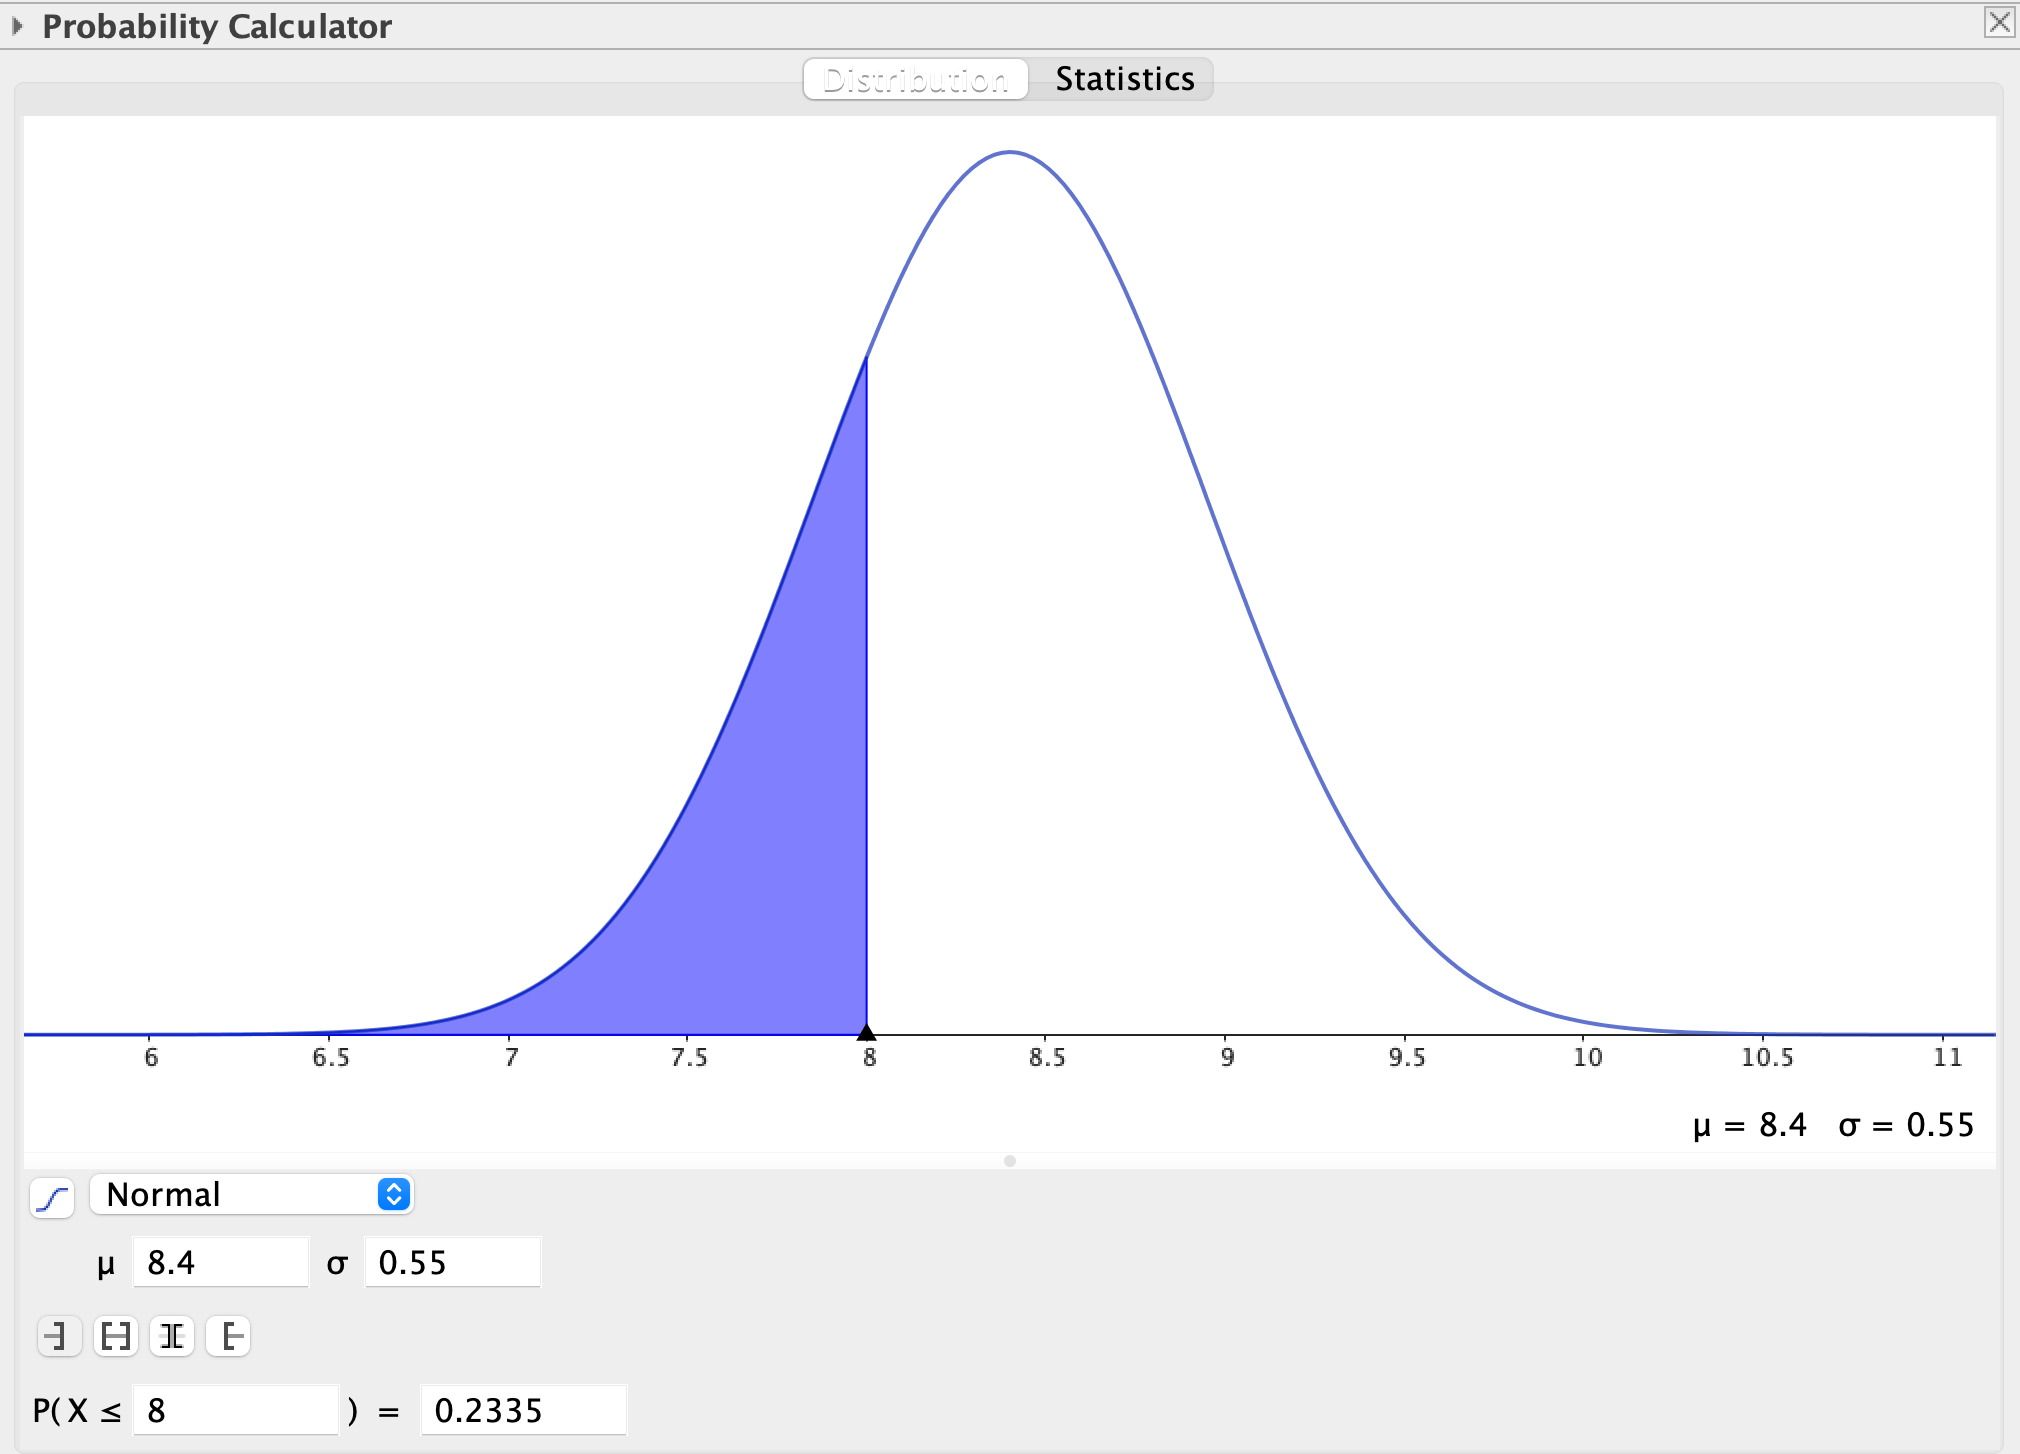
\includegraphics[width=0.5\textwidth]{CASleq8.png}
\end{center}
\caption{Sandsynligheden udregnet med CAS}
\label{fig:CASleq8}
\end{figure}

\begin{question}{Endnu en normalfordelt stokastisk variabel}{}
  En normalfordelt stokastisk variabel $X$ er givet ved $X \sim N(3,2)$.
\end{question}
\sol \\
\textbf{a.}
Grafen for fordelingsfunktionen hørende til $X$ ses i \cref{fig:fordeling}.
\begin{figure}[H]
\begin{center}
  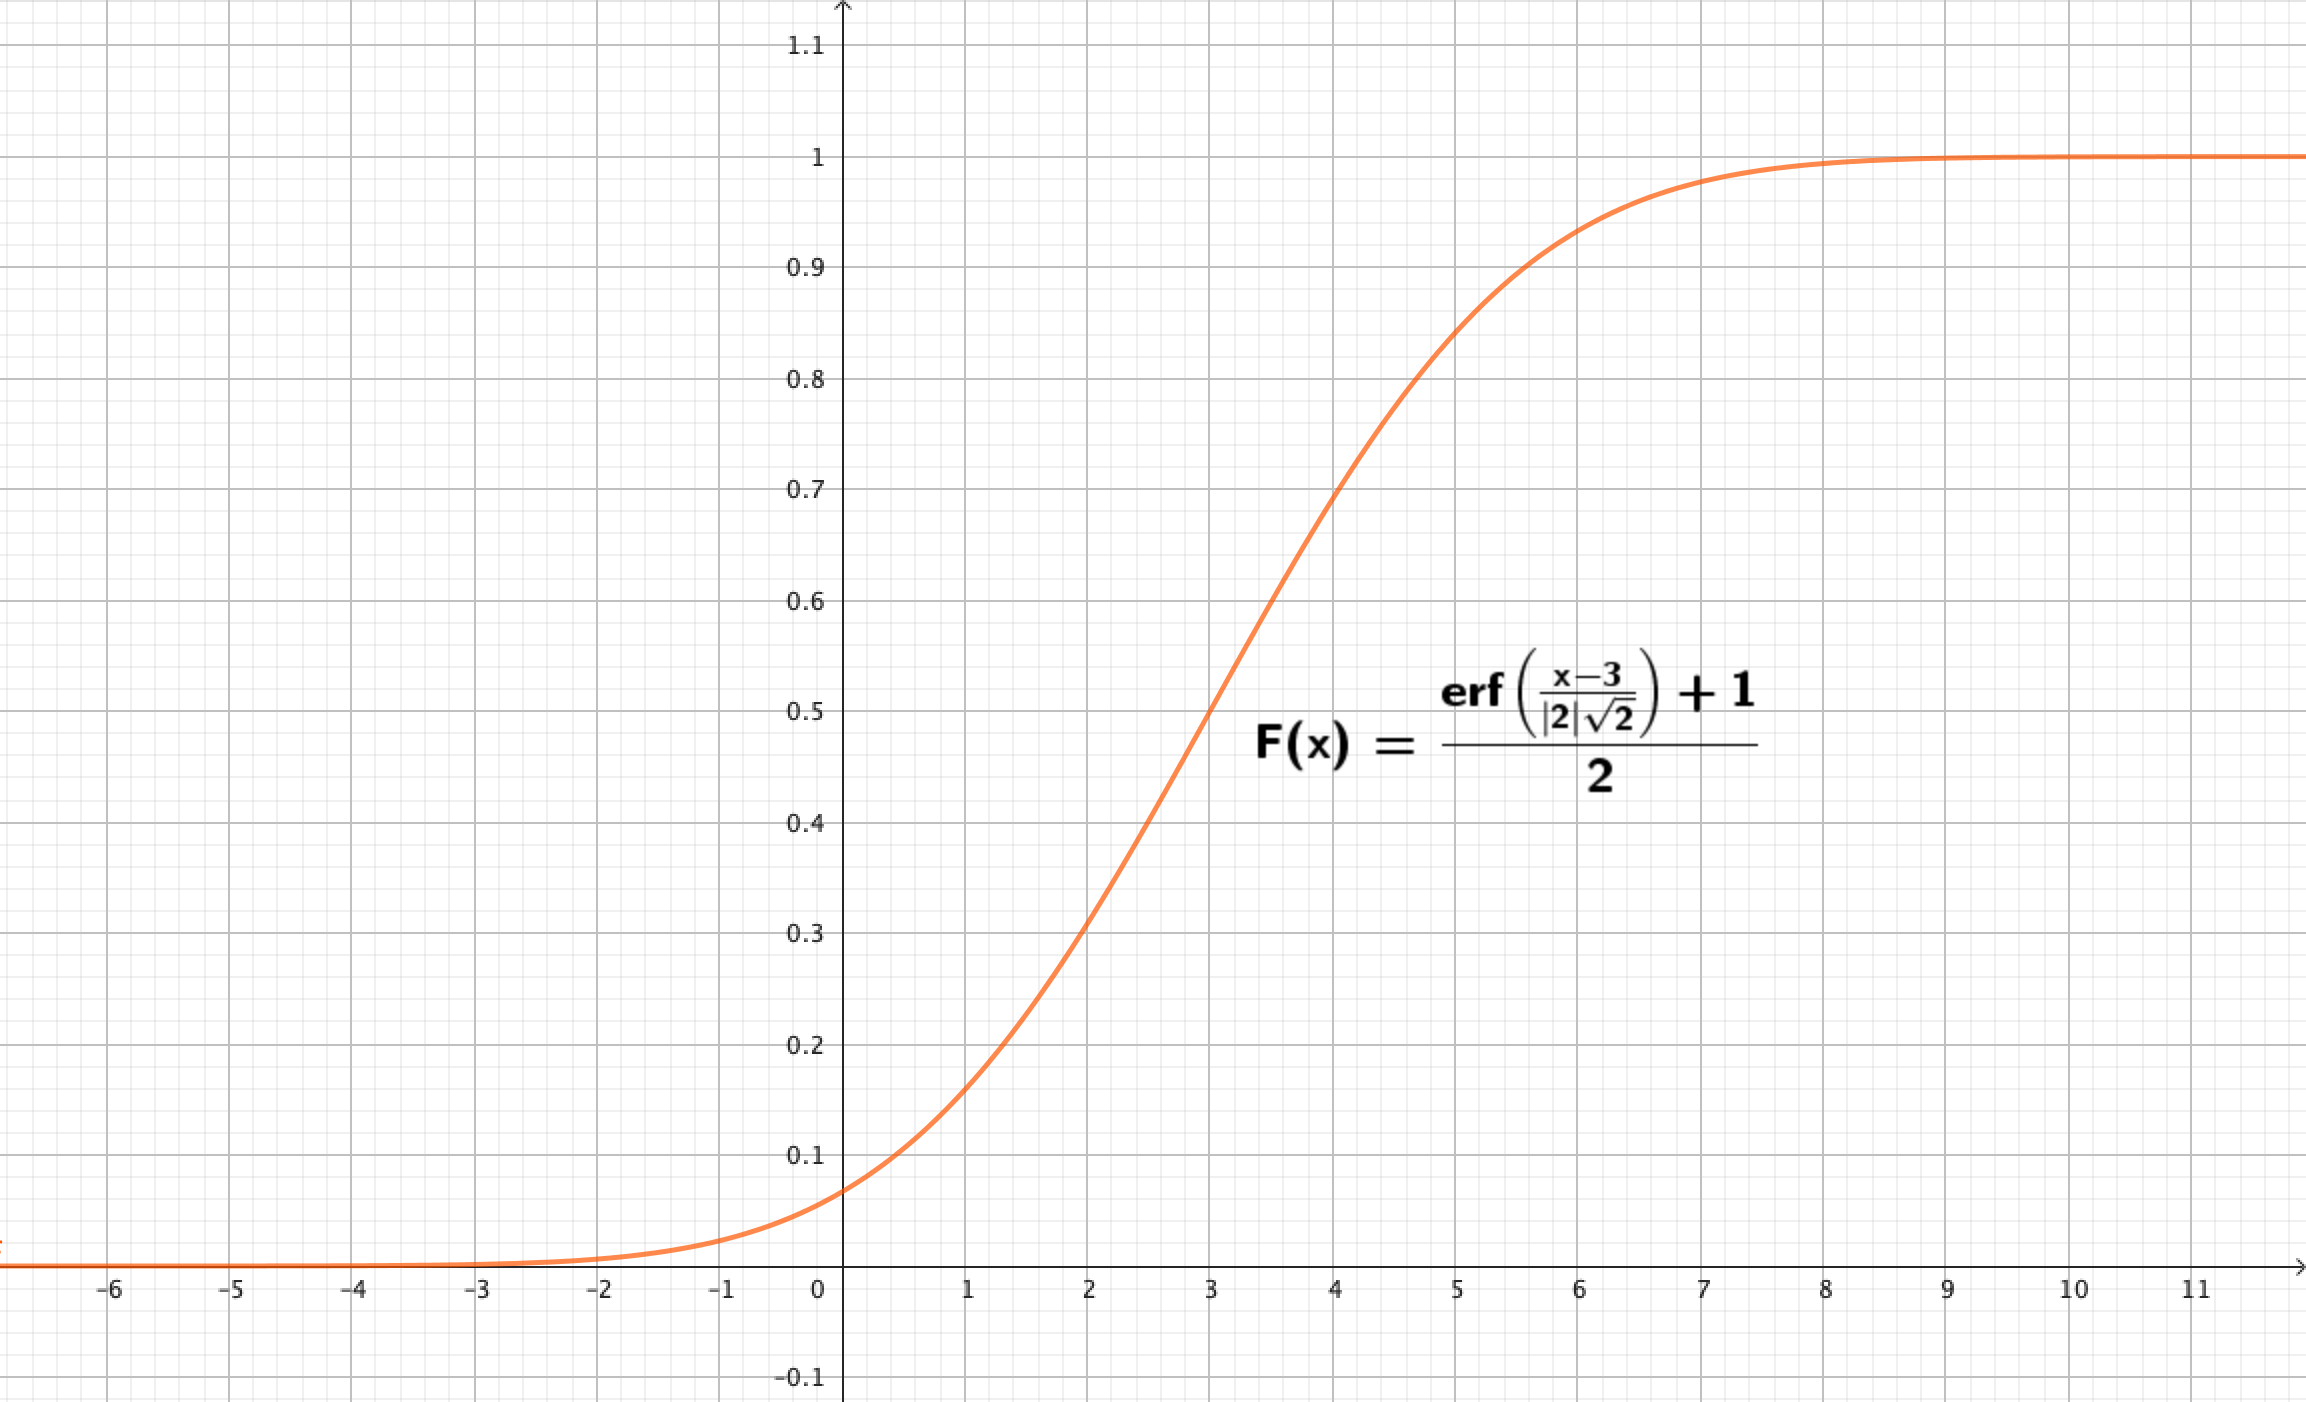
\includegraphics[width=\textwidth]{fordeling.png}
\end{center}
\caption{Graf for fordelingsfunktionen hørende til $X$}
\label{fig:fordeling}
\end{figure}
\noindent \textbf{b.}
$P(0,5 \leq X \leq 4)$ udregnes med CAS, hvilket ses i \cref{fig:CASleq4}, og vi får
\begin{equation*}
\begin{split}
P(0,5 \leq X \leq 4) \approx 0,5858
\end{split}
\end{equation*}
Altså har vi bestemt $P(0,5 \leq X \leq 4)$ til at være $0,5858$. 
\begin{figure}[H]
\begin{center}
  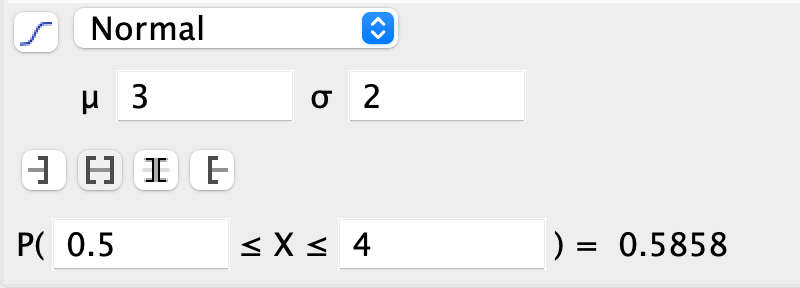
\includegraphics[width=0.5\textwidth]{CASleq4.png}
\end{center}
\caption{Sandsynligheden udregnet med CAS}
\label{fig:CASleq4}
\end{figure}
\noindent \textbf{c.}
For at bestemme $k$ benytter vi fraktilfunktionen. 
Lad $F$ betegne fordelingsfunktionen hørende til $X$ (bemærk $F$ er injektiv), så gælder
\begin{equation*}
\begin{split}
  P(X \leq k)=0,6 &\iff F(k)=0,6 \\
  &\iff k=F ^{-1}(0,6)
\end{split}
\end{equation*}
Vi beregner $F ^{-1}(0,6)$ med CAS, hvilket ses i \cref{fig:fraktilfunk}. 
\begin{equation*}
\begin{split}
  k&=F ^{-1}(0,6)\\
  &\approx 3,5067
\end{split}
\end{equation*}
Når $P(X \leq k)=0,6$, så er tallet $k$ altså $3,5067$.
\begin{figure}[H]
\begin{center}
  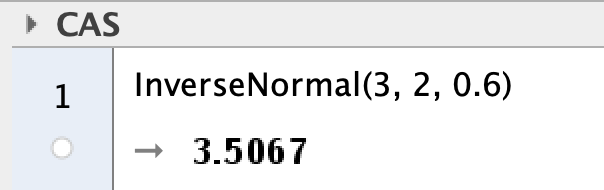
\includegraphics[width=0.5\textwidth]{fraktilfunk.png}
\end{center}
  \caption{$F ^{-1} (0.6)$ udregnet med CAS }
\label{fig:fraktilfunk}
\end{figure}
\begin{question}{Fart på en bil}{}
  I en model kan bilernes fart (målt i km/t) på en bestemt vejrstrækning beskrives ved en normalfordelt stokastisk variabel $X$ med middelværdi $\mu = 76,1$ og spredning $\sigma = 7,2$. 
  Fartgrænsen på vejrstrækningen er 80 km/t.
\end{question}
\sol \\
\textbf{a.}
Andelen af biler hurtigere end fartgrænsen må være
\begin{equation*}
\begin{split}
  P(X \geq 80)&= 1 - \Phi \left(\frac{80 - \mu }{\sigma }\right) \\
  &=1-\int_{- \infty }^{\frac{80-76,1}{7,2}}\left(  \frac{e^{-\frac{x^2}{2}} }{\sqrt{2 \pi } }\right) \,dx \\
  &\approx 0,2940\\
  &=29,40 \;\%
\end{split}
\end{equation*}
Sandsynligheden er udregnet med CAS, hvilket ses i \cref{fig:CASgeq80}.
Altså kører $29,40 \;\%$ af bilerne ifølge modellen hurtigere end de tilladte $80 \;\unit{km/t} $. 
\begin{figure}[H]
\begin{center}
  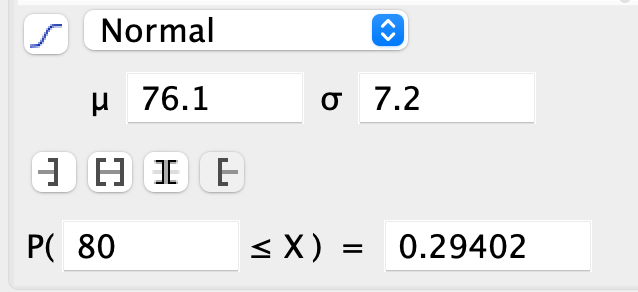
\includegraphics[width=0.5\textwidth]{CASgeq80.png}
\end{center}
\caption{Sandsynligheden udregnet med CAS}
\label{fig:CASgeq80}
\end{figure}
\noindent \textbf{c.}
For at bestemme, hvor hurtigt de hurtigste 2 \% af bilerne kører, benytter vi fraktilfunktionen.
Den fart som disse biler mindst kører betegner vi $v$, og fordelingsfunktionen hørende til $X$ betegner vi $F$.
\begin{equation*}
\begin{split}
  P(X \geq v) = 0,02 &\iff P(X \leq v) = 0,98 \\
  &\iff F(v)=0,98 \\
  &\iff v=F ^{-1}(0,98)
\end{split}
\end{equation*}
Vi beregner nu $v$ med CAS, hvilket ses i \cref{fig:CAShurtigst}. 
\begin{equation*}
\begin{split}
  v&=F ^{-1}(0,98)\\
  &\approx 90,89
\end{split}
\end{equation*}
Ifølge modellen kører de 2 \% hurtigste biler altså mindst $90,89 \;\unit{km/t} $.
\begin{figure}[H]
\begin{center}
  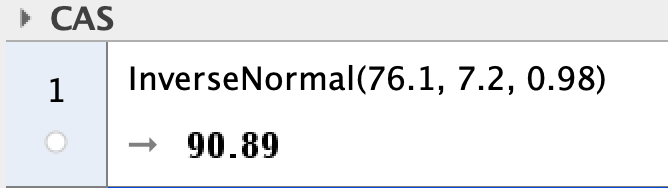
\includegraphics[width=0.5\textwidth]{CAShurtigst.png}
\end{center}
  \caption{$F ^{-1}(0,98)$ udregnet med CAS }
\label{fig:CAShurtigst}
\end{figure}
\begin{question}{Afstemning om forsvarsforbehold}{}
I en meningsmåling fra den 16. maj 2022 blandt 683 tilfældigt udvalgte danske vælgere svarede 38,2 \%, at de ville stemme nej til at ophæve det danske EU-forsvarsforbehold.

Den l. juni 2022 var der folkeafstemning om at ophæve det danske EU-forsvarsforbehold.
Ved denne folkeafstemning stemte 33,1 \% af vælgerne nej.
\end{question}
\sol \\
\textbf{a.}
Lad $\hat p $ angive stikprøveandelen af nej-svar, og $n$ være antal vælgere i meningsmålingen.
Så må 95 \% konfidensintervallet for nej-andelen af danske vælgere være 
\begin{equation*}
\begin{split}
  \left[\hat p - 2 \cdot \sqrt{\frac{\hat p \cdot (1- \hat p)}{n}} ; \hat p + 2 \cdot \sqrt{\frac{\hat p \cdot (1- \hat p)}{n}} \right]&=\left[0,382 - 2 \cdot \sqrt{\frac{0,382 \cdot (1-0,382)}{683}} ; 0,382 + 2 \cdot \sqrt{\frac{0,382 \cdot (1-0,382)}{683}} \right]\\
  &\approx \left[0,345; 0,419\right]
\end{split}
\end{equation*}
Et 95 \% konfidensinterval for nej-andelen af danske vælgere er altså $[0,345; 0,419]$.\\[1ex]
\textbf{b.}
For at bestemme, om der er sket en signifikant ændring i nej-andelen af af danske vælgere, betrager vi 95 \% konfidensintervallet fra \textbf{a.}.
Siden 
\begin{equation*}
\begin{split}
  33,1 \;\%=0,331 \notin [0,345;0,419]
\end{split}
\end{equation*}
så er der tale om en signifikant ændring.
Altså skete der en signifikant ændring i nej-andelen af danske vælgere fra den 16. maj til den 1. juni 2022.

\end{document}
